%%
%% Author: melo
%% 05/08/2018
%%

%%
%%  TODO: tabela
%%  TODO: snippet
%%  TODO: sections/enumerate/description
%%  TODO: header (only in first page)
%%  TODO: footer (all pages except on first)
%%
%%

%%%% PREAMBLE %%%%

% abntex2
\documentclass[11pt,openright,twoside,a4paper,brazil, article]{abntex2}

% Packages
\usepackage{a4wide}
\usepackage[margin=0in, ignorehead, bottom=4cm,top=2cm]{geometry}
\usepackage{lipsum}%% a garbage package you don't need except to create examples.
\usepackage{fancyhdr}
\usepackage{graphicx}
\graphicspath{ {./img/} }
\usepackage{layout} % Package that print the page dimensions (use \layout)

% New command to set text margin
\def\changemargin#1#2{\list{}{\rightmargin#2\leftmargin#1}\item[]}
\let\endchangemargin=\endlist

% Page style
\pagestyle{fancy}

\fancypagestyle{emakers}
{
    \renewcommand{\headrulewidth}{0pt}
    \fancyhf{}
    \chead{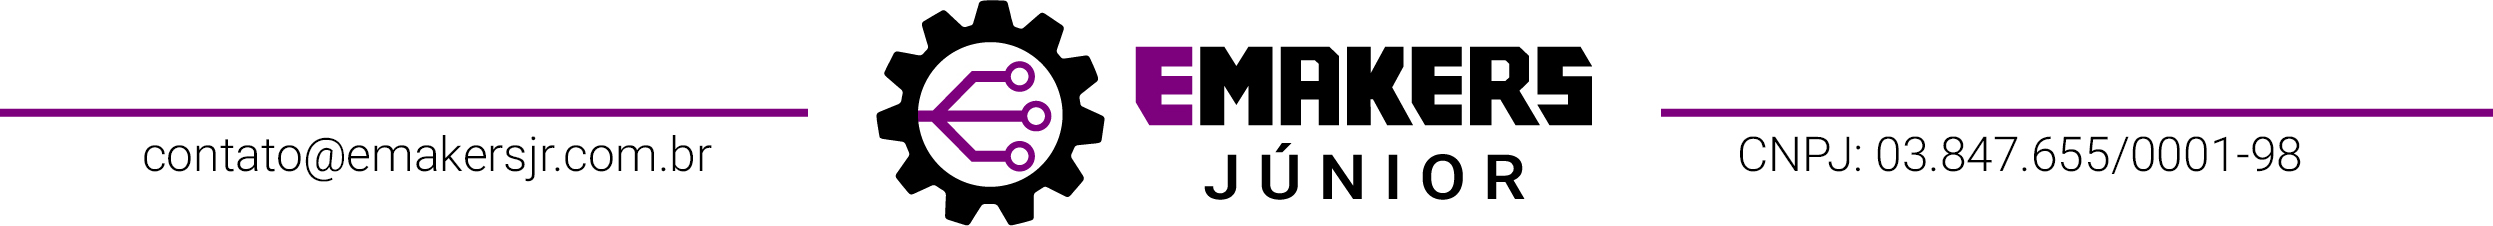
\includegraphics[scale=0.26]{header}}
    \headheight 10pt              %% put this outside
    \headsep 80pt                 %% put this outside
    \raggedbottom
}
\headheight 0pt              %% put this outside
\headsep 40pt                 %% put this outside



\title{DOCUMENT TITLE}
\author{Gabriel Marques de Melo}

% Document
\begin{document}
    \maketitle
    \thispagestyle{emakers}


    % Set text horizontal margin
    \begin{changemargin}{2cm}{2cm}
    \section{First section}\label{sec:firstSection}
        \lipsum[1]

        % FIGURE &
        \begin{figure}[!htb]
            \centering
            
\includegraphics[width=8cm]{logo-emakers}
            \caption{Emakers' logo}
            \label{logo-emakers}
        \end{figure}

        \subsection{First subsection}\label{subsec:firstSubsection}
        \lipsum[1]

    \section{Second section}\label{sec:secondSection}
        \lipsum[1]
        \subsection{teste}
            \item Este é o indice 1;
            \begin{enumerate}
                \item \lipsum[1];

            \end{enumerate}
            \item Este é o indice 1;
            \begin{enumerate}
                \item \lipsum[1];
                \item \lipsum[1];
            \end{enumerate}
    \end{changemargin}
\end{document}